\section{Time planning}

The project, initiated in July 2023, is anticipated to conclude between December and January. A single individual is allocated approximately 25 hours per week for project tasks, though this allocation may experience variations.

\subsection{Task descriptions}
In this section, we introduce the primary tasks and their corresponding subtasks, providing a brief description of each.
    \subsubsection{T1 - Project Management}
        In this initial phase, the focus will be on establishing a robust project framework.\\
        
        \textbf{T1.1 Definition of the context and project scope:}
            This phase involves clearly defining the context in which the project operates and establishing the boundaries of its scope. It includes identifying the key stakeholders, understanding the project's objectives, and delineating the specific problems or challenges it aims to address. This foundational step sets the direction for the entire project. 
            
        \textbf{T1.2 Temporal planning of the project:}
         Temporal planning focuses on creating a comprehensive schedule for the project, including task sequencing, resource allocation, and timelines. It involves setting realistic milestones and deadlines, taking into account potential project dependencies and risks. Effective temporal planning ensures efficient project management and helps keep the project on track.
         
        \textbf{T1.3 Budget and sustainability:}
        This phase entails determining the financial resources required for the project's execution, including budget allocation for various tasks and activities. Additionally, it involves a study of the project's sustainability impact, assessing its environmental, social, and economic implications. 
        
        \textbf{T1.4 Integration of Key Project Components:}
        In this stage, we integrate and consolidate the key components of the project, including the defined context and scope, the finalized temporal plan, the budget allocation, and the sustainability impact assessment. This holistic approach ensures that all project elements work seamlessly together and provides a comprehensive reference for project execution.
        
        \textbf{T1.5 Meetings with the tutor:}
        Regular meetings with the project tutor are essential for maintaining effective communication and mentorship throughout the project's lifecycle. These meetings provide opportunities to discuss progress, seek guidance, address challenges, and ensure that the project remains aligned with its objectives. Meetings with the tutor are valuable checkpoints for the project's success.
        

    \subsubsection{T2 - Design of the ILP Model}
        This phase constitutes the core of the project, involving the conceptualization and formulation of the Integer Linear Programming (ILP) model. It encompasses identifying variables, formulating constraints, and fine-tuning the model to accurately represent hypergraph orientation.\\
        
        \textbf{T2.1 Study of ILP Modeling Using AMPL:}
        Dive into the study of Integer Linear Programming (ILP) modeling principles using AMPL (A Mathematical Programming Language) as the platform. This subtask involves gaining a deep understanding of ILP concepts, syntax, and best practices for model formulation.
        
        \textbf{T2.2 Formulate the Hypergraph Model:}
        Develop an ILP model that accurately represents hypergraph orientation and obtains a solution to our optimization problem. This subtask includes identifying and defining the model's decision variables, objective function, and constraints. Ensure that the model effectively captures the complexities of hypergraph structures.
        
        \textbf{T2.3 Validation with Handcrafted Data:}
        Test the formulated ILP model using carefully crafted or synthetic hypergraph data. This subtask involves creating hypergraphs with known properties to validate the model's accuracy and functionality. 
        
        \textbf{T2.4 Testing with Real Data:}
        Apply the ILP model to real-world hypergraph data, such as metabolic pathway information from the KEGG database. This subtask assesses the model's performance and adaptability in handling practical and complex data sets.
        
        \textbf{T2.5 Benchmarking and Optimization:}
        Conduct benchmark tests to evaluate the ILP model's efficiency and scalability. Explore alternative models and solvers.

    \subsubsection{T3 - App Development:}
        Following the design of the ILP model, attention will shift towards the development of the application. This phase involves implementing the ILP model within the application framework, ensuring seamless interaction with the KEGG database, and incorporating user-friendly interfaces for efficient utilization.\\

        \textbf{T3.1 Database Interaction Setup}
        Establish robust mechanisms for the application to interact with the KEGG database, allowing for data retrieval and updates as needed.
        
        \textbf{T3.2 ILP Model Integration}
        Integrate the designed ILP model into the application's architecture, ensuring that it functions seamlessly within the software.
        
        \textbf{T3.3 Functionality Implementation}
        Implement the core functionalities of the application, ensuring that it can effectively perform hypergraph orientation tasks based on the ILP model.
        
        \textbf{T3.4 User Interface Design}
        Design and develop user-friendly interfaces for the application, focusing on usability and efficiency for end-users.
        
        \textbf{T3.5 User Documentation Creation}
        Develop comprehensive user documentation, including user guides and manuals, to assist users in effectively utilizing the application.

    \subsubsection{T4 - Implicit Task - Project Documentation:}
        Throughout the different project tasks, comprehensive documentation is an ongoing process. This includes detailing the methodology, presenting results, and providing user instructions for the application. Additionally, any supplementary materials or resources are continuously compiled for future reference.
    \subsubsection{T5 - Preparation for the oral defence}
        In the lead-up to the oral defense, thorough preparation is essential. This subtask includes finalizing the presentation materials, rehearsing the oral defense, and conducting mock presentations to ensure a confident and effective delivery during the defense session.

\begin{table}[!ht]
\centering
\begin{tabular}{|l|l|l|l|}
\hline % Draw a horizontal line at the top of the table
\rowcolor{black!25}
ID & Task & Dependencies & Duration (hours) \\ % Table header
\hline
\rowcolor{black!15}
T1 & Project Management &  & 85\\\hline
T1.1 & Definition of the context and project scope & & 25\\\hline
T1.2 & Temporal planning of the project & & 15\\\hline
T1.3 & Budget and sustainability & & 15\\\hline
T1.4 & Integration of Key Project Components & T1.1, T1.2, T1.3 & 15\\\hline
T1.5 & Meetings with the tutor & & 15\\\hline
\rowcolor{black!15}
T2 & Design of the ILP Model & & 90\\\hline
T2.1 & Study of ILP Modeling Using AMPL & & 40\\\hline
T2.2 & Formulate the Hypergraph Model& T2.1 & 15\\\hline
T2.3 & Validation with Handcrafted Data & T2.2 & 10\\\hline
T2.4 & Testing with Real Data & T2.2, T3.1 & 15\\\hline
T2.5 & Benchmarking and Optimization & T2.4 & 10\\\hline
\rowcolor{black!15}
T3 & App development & & 210\\\hline
T3.1 & Database Interaction Setup & & 35\\\hline
T3.2 & ILP Model Integration & T2.2 & 25\\\hline
T3.3 & Functionality Implementation & T3.1, T3.2& 50\\\hline
T3.4 & User Interface Design & T3.3 & 50\\\hline
T3.5 & User Documentation Creation & T3.4& 50\\\hline
\rowcolor{black!15}
T4 & Project documentation  & & 50\\\hline
\rowcolor{black!15}
T5 & Preparation for the oral defence & T1, T2, T3, T4& 30\\\hline
\multicolumn{3}{r}{Total:}& \multicolumn{1}{l}{435}

\end{tabular}
\caption{Task Duration and dependencies} % Table caption
\label{tab:TaskDurationAnddependencies}
\end{table}


\subsection{Task duration estimates}
In this section we give an estimating of the time required for the completion of tasks and subtasks. Additionally, we will identify and declare any interdependencies between these tasks where applicable. 
We provide the table \ref{tab:TaskDurationAnddependencies} which displays the durations and dependencies of the tasks. 
We also provide the figure \ref{fig:Gantt} which depicts the Gantt Chart representing the proposed workflow of the project.

\begin{landscape}
\begin{figure}[!ht]
  \centering
  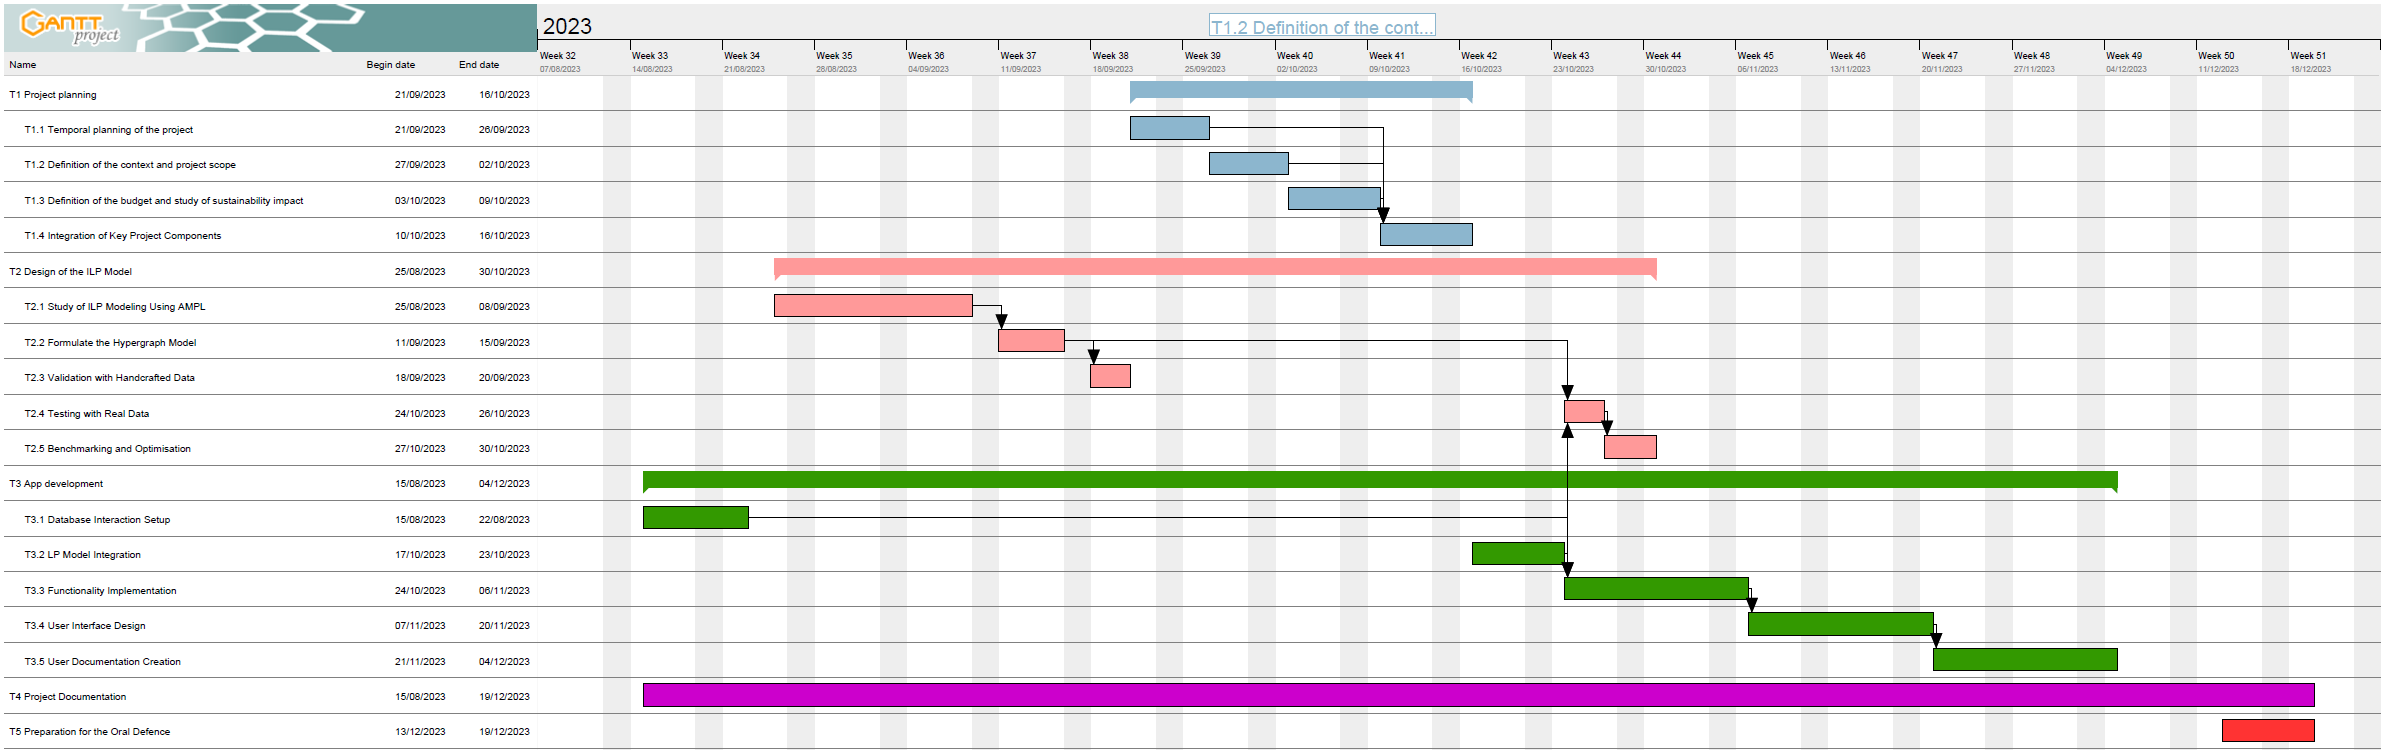
\includegraphics[scale=0.4]{GEP2/Gant.png}
  \caption{Gantt Diagram. Source : own compilation}
  \label{fig:Gantt}
\end{figure}    
\end{landscape}

\subsection{Resources}
In the pursuit of this research endeavor, several essential resources, both human and material, play a crucial role in facilitating the project's success. These resources are integral to the project's development, documentation, and overall execution.
\subsubsection{Human Resources:}
\label{sec:human_resources}
In this section, we introduce the team members working on this project and outline their roles and responsibilities:

\begin{itemize}
    \item \hypertarget{ht:author}{}\textbf{Main Developer (Author):} The principal architect of this project, the author is responsible for the project's design, development, and execution.

    \item \hypertarget{ht:supervisor}{}\textbf{University Thesis Supervisor:} The invaluable guidance and mentorship provided by the university thesis supervisor are instrumental in shaping the project's direction and ensuring academic rigor.

    \item \hypertarget{ht:GEPtutor}{}\textbf{GEP Tutor:} The GEP (GESTIÓ DE PROJECTES) tutor contributes to the project by offering instructions and feedback on the project management aspect of the research.
\end{itemize}

We have identified five distinct roles, and assigned specific responsibilities within the project:

\begin{enumerate}
    \item \textbf{Junior Project Manager:}\\
    Responsibilities: Project coordination, task scheduling, and overall project management.\\
    Assigned team member: \hyperlink{ht:author}{Author}
    \item \textbf{Project Manager:}\\
    Responsibilities: Project supervision, guidance, research leadership, methodology development, and academic oversight.\\
    Assigned team members: \hyperlink{ht:supervisor}{Thesis supervisor}, \hyperlink{ht:GEPtutor}{GEP tutor}
    \item \textbf{Junior Researcher:}\\
    Responsibilities: Research tasks, studying hypergraphs and AMPL modeling.\\
    Assigned team member: \hyperlink{ht:author}{Author}
    \item \textbf{Senior Researcher:}\\
    Responsibilities: Research and academic guidance, leadership, methodology development.\\
    Assigned team member: \hyperlink{ht:supervisor}{Thesis supervisor}
    \item \textbf{Junior Full Stack Developer:}\\
    Responsibilities: Software development, programming, and application design.\\
    Assigned team member: \hyperlink{ht:author}{Author}
\end{enumerate}

\subsubsection{Material Resources:}\label{sec:material_resources}

\hypertarget{ht:overleaf}{}\textbf{Overleaf:} A collaborative LaTeX platform, Overleaf simplifies project documentation, enabling efficient collaboration and progress tracking with the project team. \\
\hypertarget{ht:atenea}{}\textbf{Atenea:} The university's Atenea platform serves as a communication hub, providing instructions and feedback from the GEP tutor. \\
\hypertarget{ht:pycharm}{}\textbf{PyCharm IDE:} A top-tier Python Integrated Development Environment (IDE) empowers the author with advanced programming capabilities, streamlining development tasks.\\
\hypertarget{ht:chatgpt}{}\textbf{ChatGPT:} A versatile AI tool, ChatGPT assists in text composition and programming tasks, ensuring the generation of grammatically correct and comprehensive text.\\
\hypertarget{ht:amplide}{}\textbf{AMPL IDE:} The AMPL Integrated Development Environment is employed for the development and testing of AMPL (A Mathematical Programming Language) models, a critical component of the project.\\
\hypertarget{ht:github}{}\textbf{GitHub:} A robust version control platform, GitHub facilitates collaborative coding, version management, and project organization.\\
\hypertarget{ht:hpc}{}\textbf{High-Performance Computer:} Equipped with a formidable Ryzen 7 5800x3D CPU, 32GB RAM operating at 3600MHz, and an AMD Radeon RX 6900XT GPU, this high-performance computer serves as the primary development environment. In the event that this setup proves insufficient for computational demands, access to the Department of Computer Science's supercomputer cluster may be requested.

\begin{landscape}
    \begin{table}[!ht]
    \centering
    \begin{tabular}{|l|p{5cm}|l|l|}
        \hline
        \rowcolor{black!25}
        ID & Task & Roles  & Material Resource \\ \hline
        \rowcolor{black!15}
        T1 & Project Management & Junior Project Manager, Project Manager & \hyperlink{ht:overleaf}{Overleaf}, \hyperlink{ht:atenea}{Atenea}, \hyperlink{ht:chatgpt}{ChatGPT}, \hyperlink{ht:hpc}{High-Performance Computer} \\ \hline
        T1.1 & Definition of the context and project scope & Junior Project Manager, Project Manager & \hyperlink{ht:overleaf}{Overleaf}, \hyperlink{ht:atenea}{Atenea}, \hyperlink{ht:chatgpt}{ChatGPT}, \hyperlink{ht:hpc}{High-Performance Computer} \\ \hline
        T1.2 & Temporal planning of the project & Junior Project Manager, Project Manager & \hyperlink{ht:overleaf}{Overleaf}, \hyperlink{ht:atenea}{Atenea}, \hyperlink{ht:chatgpt}{ChatGPT}, \hyperlink{ht:hpc}{High-Performance Computer} \\ \hline
        T1.3 & Definition of the budget and study of sustainability impact & Junior Project Manager, Project Manager & \hyperlink{ht:overleaf}{Overleaf}, \hyperlink{ht:atenea}{Atenea}, \hyperlink{ht:chatgpt}{ChatGPT}, \hyperlink{ht:hpc}{High-Performance Computer} \\ \hline
        T1.4 & Integration of Key Project Components & Junior Project Manager, Project Manager & \hyperlink{ht:overleaf}{Overleaf}, \hyperlink{ht:atenea}{Atenea}, \hyperlink{ht:chatgpt}{ChatGPT}, \hyperlink{ht:hpc}{High-Performance Computer} \\ \hline
        T1.5 & Meetings with the tutor & All roles & ~ \\ \hline
        \rowcolor{black!15}
        T2 & Design of the ILPModel & Junior Researcher & \hyperlink{ht:amplide}{AMPL IDE}, \hyperlink{ht:hpc}{High-Performance Computer} \\ \hline
        T2.1 & Study of ILP Modeling Using AMPL & Junior Researcher & ~ \\ \hline
        T2.2 & Formulate the Hypergraph Model & Junior Researcher & \hyperlink{ht:amplide}{AMPL IDE}, \hyperlink{ht:hpc}{High-Performance Computer} \\ \hline
        T2.3 & Validation with Handcrafted Data & Junior Researcher & \hyperlink{ht:amplide}{AMPL IDE}, \hyperlink{ht:hpc}{High-Performance Computer} \\ \hline
        T2.4 & Testing with Real Data & Junior Researcher & \hyperlink{ht:amplide}{AMPL IDE}, \hyperlink{ht:hpc}{High-Performance Computer} \\ \hline
        T2.5 & Benchmarking and Optimization & Junior Researcher & \hyperlink{ht:amplide}{AMPL IDE}, \hyperlink{ht:hpc}{High-Performance Computer} \\ \hline
        \rowcolor{black!15}
        T3 & App development & Junior Full Stack Developer & \hyperlink{ht:github}{GitHub}, \hyperlink{ht:pycharm}{PyCharm IDE}, \hyperlink{ht:chatgpt}{ChatGPT}, \hyperlink{ht:hpc}{High-Performance Computer} \\ \hline
        T3.1 & Database Interaction Setup & Junior Full Stack Developer & \hyperlink{ht:github}{GitHub}, \hyperlink{ht:pycharm}{PyCharm IDE}, \hyperlink{ht:chatgpt}{ChatGPT}, \hyperlink{ht:hpc}{High-Performance Computer} \\ \hline
        T3.2 & ILP Model Integration & Junior Full Stack Developer & \hyperlink{ht:github}{GitHub}, \hyperlink{ht:pycharm}{PyCharm IDE}, \hyperlink{ht:chatgpt}{ChatGPT}, \hyperlink{ht:hpc}{High-Performance Computer} \\ \hline
        T3.3 & Functionality Implementation & Junior Full Stack Developer & \hyperlink{ht:github}{GitHub}, \hyperlink{ht:pycharm}{PyCharm IDE}, \hyperlink{ht:chatgpt}{ChatGPT}, \hyperlink{ht:hpc}{High-Performance Computer} \\ \hline
        T3.4 & User Interface Design & Junior Full Stack Developer & \hyperlink{ht:github}{GitHub}, \hyperlink{ht:pycharm}{PyCharm IDE}, \hyperlink{ht:chatgpt}{ChatGPT}, \hyperlink{ht:hpc}{High-Performance Computer} \\ \hline
        T3.5 & User Documentation Creation & Junior Full Stack Developer & \hyperlink{ht:github}{GitHub}, \hyperlink{ht:pycharm}{PyCharm IDE}, \hyperlink{ht:chatgpt}{ChatGPT}, \hyperlink{ht:hpc}{High-Performance Computer} \\ \hline
        \rowcolor{black!15}
        T4 & Project documentation & Junior Full Stack Developer & \hyperlink{ht:chatgpt}{ChatGPT} \\ \hline
        \rowcolor{black!15}
        T5 & Preparation for the oral defence & Junior Researcher, Junior Full Stack Developer & \hyperlink{ht:chatgpt}{ChatGPT} \\ \hline
    \end{tabular}
    \caption{Table of requirements (Human and Material) corresponding to each task}
    \label{tab:requirementsHRMat}
\end{table}
\end{landscape}

\subsection{Risk Management: Obstacles and alternative plans}
In the pursuit of this research project, we have identified several potential risks that may affect its execution. In this section, we discuss these risks, propose solutions, and provide estimates of possible consequences in terms of additional time and resources required.\\
\subsubsection{Project Timeline}

    \textbf{Risk:} Some tasks may have been underestimated and may take longer than expected for various reasons.\\
    \textbf{Proposed Solution:} It is crucial to monitor our progress and be aware of the expected development stage at any given time. This enables us to adjust our plans if necessary.\\
    \textbf{Possible Consequences:} In the worst-case scenario, we may require an additional 50 to 80 hours of labor.\\
    \textbf{Probability:} Low. We have already conducted a comprehensive field study during the document's preparation, allowing us to identify potential obstacles and adapt the project plan and scope accordingly.
    
\subsubsection{Computational power}

    \textbf{Risk:} The computer we have may not be powerful enough to handle the largest hypergraphs efficiently.\\
    \textbf{Proposed Solution:} In case our current setup proves insufficient, we will establish contact with the computing cluster of the Department of Computer Science to process more demanding cases.\\
    \textbf{Possible Consequences:} In the event of computational limitations, there might be a delay of multiple days. During this time, Task T2.4 might be affected. However, our project plan allows us to proceed with different tasks that do not rely on T2.4 as a predecessor. At worst, we anticipate a delay of 15 hours.\\
    \textbf{Probability:} Low. Early testing shows that the computer at our dispositions is sufficiently powerful.
    
\subsubsection{Integration Challenges}

\textbf{Risk:} Integration with the KEGG database may present challenges, including content and format discrepancies.\\
\textbf{Proposed Solution:} To address integration challenges effectively, we will implement the following strategies:\\
- Stay informed about updates to the KEGG database.\\
- Establish communication channels with the KEGG team if possible.\\
- Develop a flexible application architecture capable of accommodating changes as they occur.\\
\textbf{Possible Consequences:} Integration challenges may lead to additional effort and time spent on data processing and application adaptation. The extent of the consequences will depend on the nature and frequency of changes in the KEGG database. We expect a delay of up two 50 hours.\\
\textbf{Probability:} High. We have already identified several shortcomings in the data available that could impact Tasks T3.3 and T3.4.

\subsubsection{Inexperience with ILP:}

\textbf{Risk:} The author's limited experience with Integer Linear Programming (ILP) poses a potential challenge.\\
\textbf{Proposed Solution:} To overcome inexperience with ILP, we will adopt a proactive approach that includes:\\
    - Utilizing educational resources, such as online courses and textbooks.\\
    - Seeking guidance and mentorship from experts in the field.\\
    - Engaging in practical exercises to apply ILP concepts.\\
    - Collaborating with individuals experienced in ILP.\\
    - Committing to continuous learning throughout the project.\\
\textbf{Possible Consequences:} While there may be an initial learning curve, dedicating time and effort to gaining proficiency in ILP should mitigate potential challenges related to inexperience.
Some tasks may have been underestimated and may take longer than expected for various reasons. We may expect up to extra 20 hours.\\
\textbf{Probability:} Low. We already have a working model. 

